\documentclass[aspectratio=169]{../latex_main/tntbeamer}  % you can pass all options of the beamer class, e.g., 'handout' or 'aspectratio=43'
\usepackage{dsfont}
\usepackage{bm}
\usepackage[english]{babel}
\usepackage[T1]{fontenc}
%\usepackage[utf8]{inputenc}
\usepackage{graphicx}
\graphicspath{ {./figures/} }
\usepackage{algorithm}
\usepackage[ruled,vlined,algo2e,linesnumbered]{algorithm2e}
\usepackage{hyperref}
\usepackage{booktabs}
\usepackage{mathtools}

\usepackage{amsmath,amssymb}

\DeclareMathOperator*{\argmax}{arg\,max}
\DeclareMathOperator*{\argmin}{arg\,min}

\usepackage{amsbsy}
\newcommand{\vect}[1]{\bm{#1}}
%\newcommand{\vect}[1]{\boldsymbol{#1}}

\usepackage{pgfplots}
\pgfplotsset{compat=1.16}
\usepackage{tikz}
\usetikzlibrary{trees} 
\usetikzlibrary{shapes.geometric}
\usetikzlibrary{positioning,shapes,shadows,arrows,calc,mindmap}
\usetikzlibrary{positioning,fadings,through}
\usetikzlibrary{decorations.pathreplacing}
\usetikzlibrary{intersections}
\pgfdeclarelayer{background}
\pgfdeclarelayer{foreground}
\pgfsetlayers{background,main,foreground}
\tikzstyle{activity}=[rectangle, draw=black, rounded corners, text centered, text width=8em]
\tikzstyle{data}=[rectangle, draw=black, text centered, text width=8em]
\tikzstyle{myarrow}=[->, thick, draw=black]

% Define the layers to draw the diagram
\pgfdeclarelayer{background}
\pgfdeclarelayer{foreground}
\pgfsetlayers{background,main,foreground}

% Requires XeLaTeX or LuaLaTeX
%\usepackage{unicode-math}

\usepackage{fontspec}
%\setsansfont{Arial}
\setsansfont{RotisSansSerifStd}[ 
Path=../latex_main/fonts/,
Extension = .otf,
UprightFont = *-Regular,  % or *-Light
BoldFont = *-ExtraBold,  % or *-Bold
ItalicFont = *-Italic
]
\setmonofont{Cascadia Mono}[
Scale=0.8
]

% scale factor adapted; mathrm font added (Benjamin Spitschan @TNT, 2021-06-01)
%\setmathfont[Scale=1.05]{Libertinus Math}
%\setmathrm[Scale=1.05]{Libertinus Math}

% other available math fonts are (not exhaustive)
% Latin Modern Math
% XITS Math
% Libertinus Math
% Asana Math
% Fira Math
% TeX Gyre Pagella Math
% TeX Gyre Bonum Math
% TeX Gyre Schola Math
% TeX Gyre Termes Math

% Literature References
\newcommand{\lit}[2]{\href{#2}{\footnotesize\color{black!60}[#1]}}

%%% Beamer Customization
%----------------------------------------------------------------------
% (Don't) Show sections in frame header. Options: 'sections', 'sections light', empty
\setbeamertemplate{headline}{empty}

% Add header logo for normal frames
\setheaderimage{
	% 
\includegraphics[height=\logoheight]{figures/TNT_darkv4.pdf}
	
\includegraphics[height=\logoheight]{../latex_main/figures/luh_logo_rgb_0_80_155.pdf}
	% 
\includegraphics[height=\logoheight]{figures/logo_tntluh.pdf}
}

% Header logo for title page
\settitleheaderimage{
	% 
\includegraphics[height=\logoheight]{figures/TNT_darkv4.pdf}
	
\includegraphics[height=\logoheight]{../latex_main/figures/luh_logo_rgb_0_80_155.pdf}
	% 
\includegraphics[height=\logoheight]{figures/logo_tntluh.pdf}
}

% Title page: tntdefault 
\setbeamertemplate{title page}[tntdefault]  % or luhstyle
% Add optional title image here
%\addtitlepageimagedefault{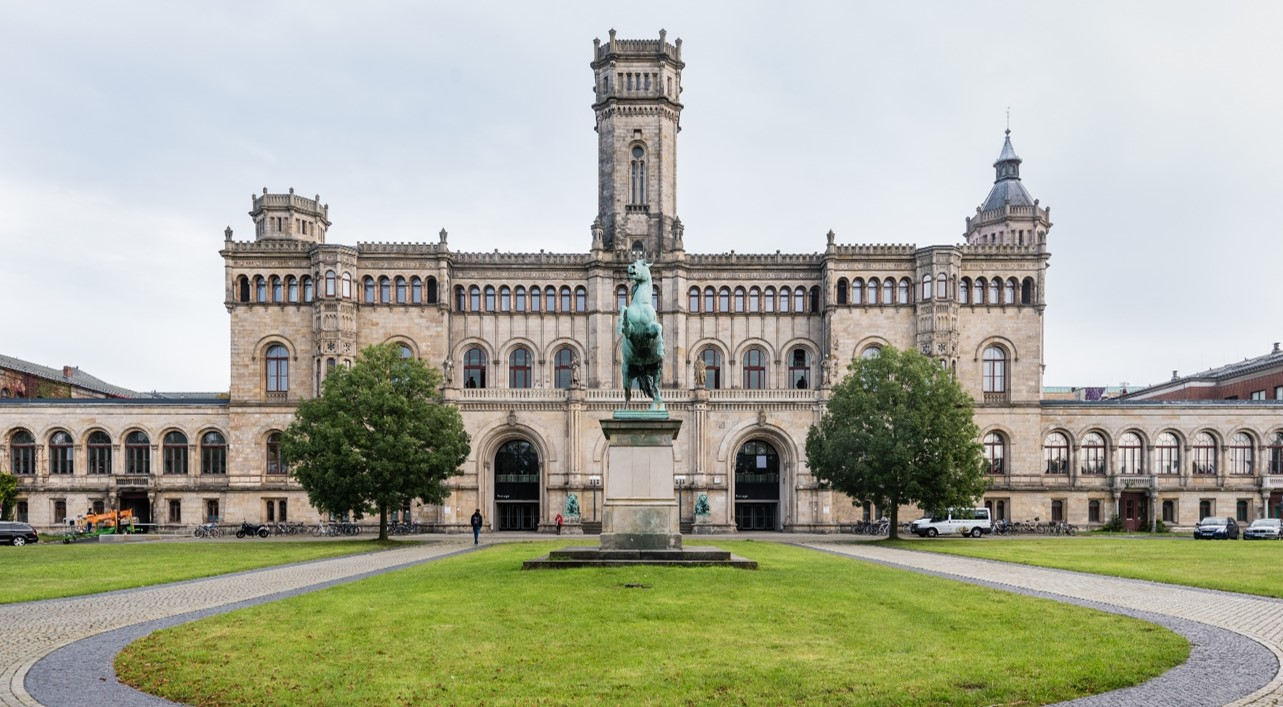
\includegraphics[width=0.65\textwidth]{figures/luh_default_presentation_title_image.jpg}}

% Title page: luhstyle
% \setbeamertemplate{title page}[luhstyle]
% % Add optional title image here
% \addtitlepageimage{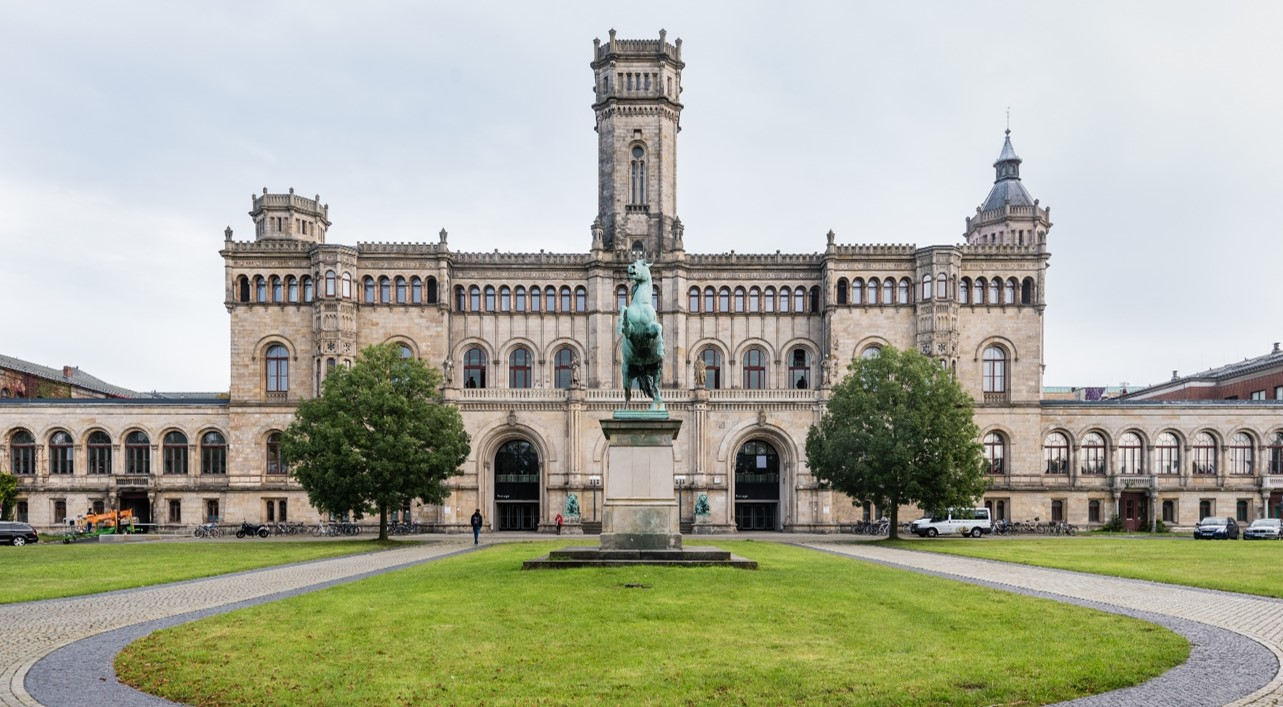
\includegraphics[width=0.75\textwidth]{figures/luh_default_presentation_title_image.jpg}}

\author[Abedjan \& Lindauer]{Ziawasch Abedjan \& Marius Lindauer\\[1em]
	
\includegraphics[height=\logoheight]{../latex_main/figures/luh_logo_rgb_0_80_155.pdf}\qquad
	
\includegraphics[height=\logoheight]{../latex_main/figures/DBIS_Kurzlogo.png}\qquad

\includegraphics[height=\logoheight]{../latex_main/figures/TNT_darkv4}\qquad

\includegraphics[height=\logoheight]{../latex_main/figures/L3S.jpg}	}
\date{Summer Term 2022; \hspace{0.5em} {
\includegraphics[height=1.5em]{../latex_main/figures/Cc-by-nc-sa_icon.svg.png}}; based on \href{https://ds100.org/fa21/}{[DS100]}
}


%%% Custom Packages
%----------------------------------------------------------------------
% Create dummy content
\usepackage{blindtext}

% Adds a frame with the current page layout. Just call \layout inside of a frame.
\usepackage{layout}


%%% Macros
%\renewcommand{\vec}[1]{\mathbf{#1}}
% \usepackage{bm}
%\let\vecb\bm

\title[Introduction]{DS: Cross-Validation and Regularization}
\subtitle{Ridge and LASSO Regression}

\graphicspath{ {./figure/} }
%\institute{}


\begin{document}
	
	\maketitle
	\begin{frame}{Ridge Regression}
	    “Ridge Regression” is a term for the following specific combination of model, loss, and regularization:
	    \begin{itemize}
	        \item Model: $\mathbb{\hat{Y}} = \mathbb{X}\hat{\theta}$
	        \item Loss: Squared loss
	        \item Regularization: L2 regularization
	    \end{itemize}
	    The objective function we minimize for Ridge Regression is average squared loss, plus an added penalty:
	    \begin{equation*}
	        \hat{\theta}_{ridge} = \underset{\theta}{\text{arg min}}\frac{1}{n}||\mathbb{Y} - \mathbb{X}\theta||_2^2 + \lambda \sum\limits_{j=1}^d\theta_i^2 
	    \end{equation*}
	\end{frame}
	
	
	\begin{frame}{Ridge Regression}
	    We can also express this objective slightly differently:
	    \begin{equation*}
	        \hat{\theta}_{ridge} = \underset{\theta}{\text{arg min}}\frac{1}{n}||\mathbb{Y} - \mathbb{X}\theta||_2^2 + \lambda \sum\limits_{j=1}^d\theta_i^2 
	    \end{equation*}
	    
	    \begin{equation*}
	        \hat{\theta}_{ridge} = \underset{\theta}{\text{arg min}}\frac{1}{n}||\mathbb{Y} - \mathbb{X}\theta||_2^2 + \lambda ||\theta ||_2^2
	    \end{equation*}
	    $||\theta ||$: L2 norm of $\theta$ (hence, L2 regularization)\\
	    \bigskip
	    The latter representation ignores the fact that we typically don’t regularize the intercept term
	\end{frame}
	
	
	\begin{frame}[c]{Ridge Regression}
	    Ridge Regression has a closed form solution, conveniently:
	    \begin{equation*}
	        \hat{\theta}_{ridge} = (\mathbb{X}^T\mathbb{X} + n\lambda I)^{-1} 
	    \end{equation*}
	    I: Identity matrix
	    Unlike OLS, there always exists a unique optimal parameter vector for Ridge Regression.\\
        This is important, you should remember it!

	\end{frame}
	
	
	\begin{frame}{LASSO  Regression}
	    “LASSO Regression” is a term for the following specific combination of model, loss, and regularization:
	    \begin{itemize}
	        \item Model: $\mathbb{\hat{Y}} = \mathbb{X}\hat{\theta}$
	        \item Loss: Squared loss
	        \item Regularization: L1 regularization
	    \end{itemize}\\
	    \bigskip
	    The objective function we minimize for LASSO  Regression is average squared loss, plus an added penalty:
	    \begin{equation*}
	        \hat{\theta}_{LASSO} = \underset{\theta}{\text{arg min}}\frac{1}{n}||\mathbb{Y} - \mathbb{X}\theta||_2^2 + \lambda \sum\limimts_{j=1}^d|\theta_i|
	    \end{equation*}
	\end{frame}
	
	
	
	\begin{frame}{LASSO  Regression}
	    We can also express this objective slightly differently:
	    \begin{equation*}
	        \hat{\theta}_{LASSO} = \underset{\theta}{\text{arg min}}\frac{1}{n}||\mathbb{Y} - \mathbb{X}\theta||_2^2 + \lambda \sum\limits_{j=1}^d|\theta_i|
	    \end{equation*}
	    
	    \begin{equation*}
	        \hat{\theta}_{LASSO} = \underset{\theta}{\text{arg min}}\frac{1}{n}||\mathbb{Y} - \mathbb{X}\theta||_2^2 + \lambda ||\theta ||_1
	    \end{equation*}
	    \bigskip
	   \\Unfortunately, there is no closed-form solution for the optimal parameter vector for LASSO. We must use numerical methods (like gradient descent).

	\end{frame}
	
	
	\begin{frame}{Summary of Regression Methods}
	   %\begin{array}{|l|l|l|l|l|l|}
	   %     \hline
	   %    Name & Model & Loss & Reg. & Objective & Solution \\
	   %    \hline 
	   %     OLS & \mathbb{\hat{Y} = \mathbb{X}\hat{\theta}} &  \text{Squared loss} & \text{None} & \frac{1}{n}||\mathbb{Y} - \mathbb{X}\hat{\theta}||^2_2 & \hat{\theta}_{OLS} = (\mathbb{X}^T\mathbb{X})^{-1}\mathbb{X}^T\mathbb{Y}\\
	   %     \hline
	   %     \text{Ridge Regression} & \mathbb{\hat{Y} = \mathbb{X}\hat{\theta}} & \text{Squared loss} & \text{L2} & \frac{1}{n}||\mathbb{Y} - \mathbb{X}\theta||_2^2 + \lambda \sum\limits_{j=1}^d\theta_i^2 & \hat{\theta}_{\text{ridge}} = (\mathbb{X}^T\mathbb{X} + n\lambda I)^{-1}\mathbb{X}^T\mathbb{Y}\\
	   %     \hline
    %         \text{LASSO}& \mathbb{\hat{Y} = \mathbb{X}\hat{\theta}} & \text{Squared loss}& \text{L1} & \frac{1}{n}||\mathbb{Y} - \mathbb{X}\theta||_2^2 + \lambda \sum\limits_{j=1}^d|\theta_i| & \text{no closed form}\\
    %         \hline
	   %\end{array}
	   
	   \begin{figure}
	       \centering
	       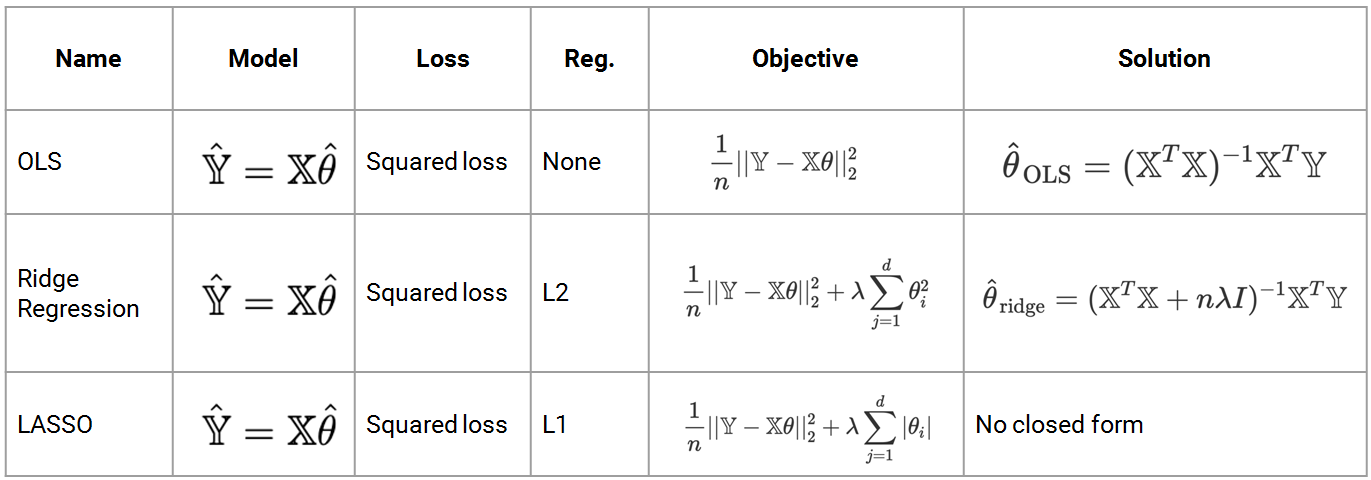
\includegraphics[scale=.4]{Bild19}
	   \end{figure}
	\end{frame}
	
	
	\begin{frame}{Fitting vs. Evaluating}
	While we may use a regularized objective function to determine our model’s parameters, we still look at (root) mean squared error to evaluate our model’s performance.
    
    \begin{equation*}
        \hat{\theta}_{ridge} = \underset{\theta}{\text{arg min}}\frac{1}{n}||\mathbb{Y} - \mathbb{X}\theta||_2^2 + \lambda \sum\limits_{j=1}^d\theta_i^2 
    \end{equation*}
    The regularization penalty is there for the purposes of model fitting only.
    \begin{equation*}
        RMSE = \sqrt{\frac{1}{n}\sum\limits_{i=1}^n(y_i - \mathbb{X}_i^T\hat{\theta}_{ridge})^2} = \sqrt{\frac{1}{n}||\mathbb{Y} - \mathbb{X}\hat{\theta}_{ridge}||_2^2}
    \end{equation*}
	\end{frame}
	
	
	\begin{frame}{Hyperparameters vs. Parameters}
        \begin{itemize}
            \item Parameters are facts about the world that we want to estimate
            \begin{itemize}
                \item Commonly denoted by p, $\theta, \theta_i$
            \end{itemize}
            \item Statistics are the estimators of the parameters, based on our data
            \begin{itemize}
                \item Commonly denoted by $\hat{p}, \hat{\theta}, \hat{\theta}_i$
            \end{itemize}
        \end{itemize}\\
        \bigskip
        Hyperparameters are design choices we make in our modeling process that affect our model, but do not directly come from the data

        \begin{itemize}
            \item examples: regularization hyperparameter, degree of polynomial
            \item Commonly denoted by $\lambda, \alpha, C$
        \end{itemize}
	\end{frame}
\end{document}